% This is the ADASS_template.tex LaTeX file, 18th Dec 2018.
% It is based on the ASP general author template file, but modified to reflect the specific
% requirements of the ADASS proceedings.
% Copyright 2014, Astronomical Society of the Pacific Conference Series
% Revision:  14 August 2014

% To compile, at the command line positioned at this folder, type:
% latex ADASS_template
% latex ADASS_template
% dvipdfm ADASS_template
% This will create a file called ADASS_template.pdf

\documentclass[11pt,twoside]{article}

% Do NOT use ANY packages other than asp2014.
\usepackage{asp2014}
%\usepackage{graphicx}

\aspSuppressVolSlug
\resetcounters

% References must all use BibTeX entries in a .bibfile.
% References must be cited in the text using \citet{} or \citep{}.
% Do not use \cite{}.
% See ManuscriptInstructions.pdf for more details
\bibliographystyle{asp2014}

% The ``markboth'' line sets up the running heads for the paper.
% 1 author: "Surname"
% 2 authors: "Surname1 and Surname2"
% 3 authors: "Surname1, Surname2, and Surname3"
% >3 authors: "Surname1 et al."
% Replace ``Short Title'' with the actual paper title, shortened if necessary.
% Use mixed case type for the shortened title
% Ensure shortened title does not cause an overfull hbox LaTeX error
% See ASPmanual2010.pdf 2.1.4  and ManuscriptInstructions.pdf for more details
\markboth{Joliet}{Control a telescope with Firefly}

\begin{document}

\title{Control any telescope with Firefly visualization tool and machine learning}

% Note the position of the comma between the author name and the
% affiliation number.
% Authors surnames should come after first names or initials, eg John Smith, or J. Smith.
% Author names should be separated by commas.
% The final author should be preceded by "and".
% Affiliations should not be repeated across multiple \affil commands. If several
% authors share an affiliation this should be in a single \affil which can then
% be referenced for several author names. If only one affiliation, no footnotes are needed.
% See ManuscriptInstructions.pdf and ASP's manual2010.pdf 3.1.4 for more details
\author{Emmanuel~Joliet}
\affil{$^1$IPAC/Caltech, Pasadena, CA, USA; \email{ejoliet@caltech.edu}}

%\author{Sample~Author1,$^1$ Sample~Author2,$^2$ and Sample~Author3$^2$}
%\affil{$^1$Institution Name, Institution City, State/Province, Country; \email{AuthorEmail@email.edu}}
%\affil{$^2$Institution Name, Institution City, State/Province, Country}

% This section is for ADS Processing.  There must be one line per author. paperauthor has 9 arguments.
\paperauthor{Emmanuel~Joliet}{ejoliet@ipac.caltech.edu}{}{California Institute of Technology}{IPAC}{Pasadena}{California}{91125}{USA}

%\paperauthor{Sample~Author1}{Author1Email@email.edu}{ORCID_Or_Blank}{Author1 Institution}{Author1 Department}{City}{State/Province}{Postal Code}{Country}
%\paperauthor{Sample~Author2}{Author2Email@email.edu}{ORCID_Or_Blank}{Author2 Institution}{Author2 Department}{City}{State/Province}{Postal Code}{Country}
%\paperauthor{Sample~Author3}{Author3Email@email.edu}{ORCID_Or_Blank}{Author3 Institution}{Author3 Department}{City}{State/Province}{Postal Code}{Country}

% There should be one \aindex line (commented out) for each author. These are used to
% build up the author index for the Proceedings. The surname must come first, followed by
% initials. Note the use of ~ before each initial to control spacing.
% The \author entries (see above) have surname last. These \aindex entries have
% surname first.
% The Aindex.py command willl create them for you after you have constructed the \author

%\aindex{Joliet,~E.}

\newcommand{\code}[1]{\texttt{#1}}

\begin{abstract}
Caltech/IPAC Firefly astronomical visualization software was used as a Python client to control the pointing of a telescope.
During Caltech Astroinformatics 2019 Hackathon, i worked on a project proposed by Alberto Krone-Martins and came up with the idea to extend the project using Firefly as a feature-rich visualization tool to enhance the observing experience.
The original hackathon project idea was about improving and making more accurate the autonomous telescope and satellite control pointing using machine learning from a training set of few images to eliminate the 'noise' coming from the control system.
Once the control loop is complete and working, the observer could use Firefly to select the target and activate the telescope control system to accurately point to the sky and make the observation.
The poster will explain the concepts and walk through each of the building block required to put together such system in place using docker and python. The result software stack can be found here: https://github.com/ejoliet/indi-firefly
\end{abstract}

% These lines show examples of subject index entries. At this stage these have to commented
% out, and need to be on separate lines. Eventually, they will be automatically uncommented
% and used to generate entries in the Subject Index at the end of the Proceedings volume.
% Don't leave these in! - replace them with ones relevant to your paper.
%\ssindex{FOOBAR!conference!ADASS 2018}
%\ssindex{FOOBAR!organisations!ASP}

% These lines show examples of ASCL index entries. At this stage these have to commented
% out, and need to be on separate lines. Eventually, they will be automatically uncommented
% and used to generate entries in the ASCL Index at the end of the Proceedings volume.
% The ascl.py command will scan your paper on possible code names.
% Don't leave these in! - replace them with ones relevant to your paper.
%\ooindex{FOOBAR, ascl:1101.010}


\section{The project}

The problem we propose to solve is to control accurately and automatically the telescope pointing and tracking of a target without the need of manual adjustments (structural noise, temperature, gyroscopes, etc.).
The idea came up during Caltech's Astroinformatics hackathon 2019, Alberto Krone-Martins proposed to improve the telescope pointing control using machine learning and automation loop with INDI \footnote{https://www.indilib.org} controller via Python API.
The solution envisioned was to take full advantage of feature-rich visualization client tool such as Firefly\footnote{https://github.com/Caltech-IPAC/firefly} and Python client API to control and point/measure devices compatible with INDI drivers.

The current software stack is a Docker image that includes INDI client/server hub and Firefly/INDI Python client code\footnote{https://github.com/ejoliet/indi-firefly} integrated and self contained ready to be connected to any INDI compatible devices.

\clearpage

\section{The architecture}

The architecture (see figure \ref{arch1}) used is a client/server type, where:
\begin{itemize}
  \item The server is the Instrument Neutral Distributed Interface (INDI) Central hub for communication between compatible drivers and clients
  \item The client is a Front-end software that enables the user to interact with INDI compatible devices and other clients such as dome, CCD, weather forcast services, etc.
  \item The driver is the software to control INDI device and provide/expose its properties in a standard format -> connect to physical device
\end{itemize}

The goal was to develop and include the software stack in a docker image to be easily shared and run practically anywhere.
To run the client/server, install/run docker and have access to launch Firefly client and INDI/Kstars simulators\footnote{See demo guidelines: https://github.com/ejoliet/indi-firefly/blob/master/DEMO-guide.md}

\begin{figure}[ht]
  %  \centering
%    \noindent\makebox[\textwidth]
   \includegraphics[scale=.7]{arch1.eps}
    \caption{Schema of the client/server architecture examples}
    \label{arch1}
\end{figure}

\section{Firefly}

Caltech/IPAC Firefly\footnote{https://github.com/Caltech-IPAC/firefly} is an open source Java/ReactJS library to build browser based visualization tools for astronomical data analysis and exploration and consist of 2 main mode of usage, the library can be iether imported from the result JavaScript API to build customized HTML pages or directly from Python.
Firefly Python client (\footnote{use command line 'pip install firefly\_client' to install python client})
Either way, the tools can make use of the widgets - See screenshots in figure \ref{ff} for Firefly use case examples.

IPAC contributing projects to Firefly are IRSA, NED and but other projects are using and integrating the library in their tools.

\begin{figure}[ht]
  %\centering
%    \noindent\makebox[\textwidth]
   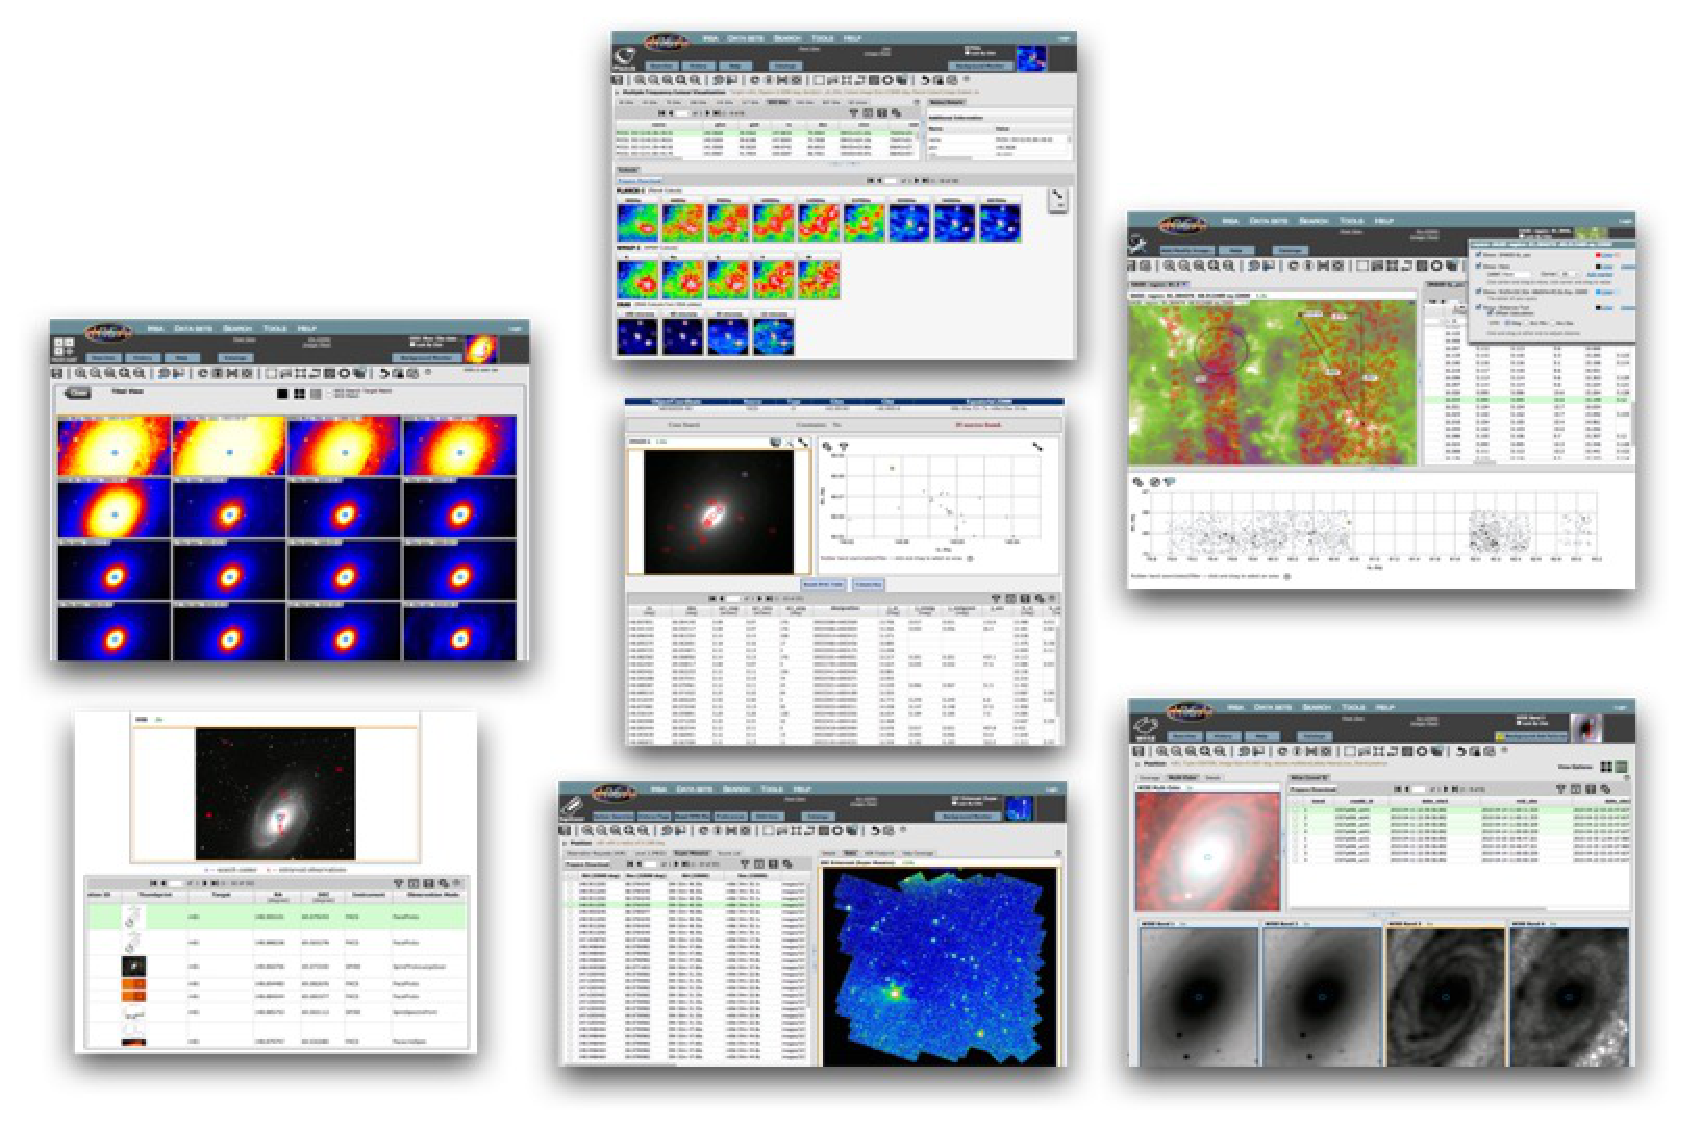
\includegraphics[scale=.5]{ff.eps}
    \caption{Firefly use case examples}
    \label{ff}
\end{figure}

\section{The client}

The client code developped during this project to control INDI compatible devices is the result of the integration of a Firefly Python client using custom callback extension and INDI client.
Kstars\footnote{https://kde.org/applications/education/org.kde.kstars} software is used to simulate INDI compatible devices such as a virtual telescope and a CCD and to visualize the tracking and the pointing of the field of view while controlling the telescope from Firefly web browser tool. See figure \ref{arch1}.

\section{Machine learning}

The idea is that before observing or tracking a target, a machine learning classifier need to be generated with the current telescope/devices setup on a sky sample.
The resulting model will represent the noise/calibration on the target position and will represent the offset tobe applied during the control loop on a real target.
In order to get the model the first step is to 'randomly' observe distributed known objects in the sky with accuarte position.

Pointing the telescope to an object and taking images will generate a 'training' set from which we can extract well-known positions. When pointing with the telescope, we can apply this offset for any susequent position target.
The ML model will include 'observer'/site/instrument/weather noise calibration unknown as part of the offset to be applied.

On every target pointing, we would run through the ML model that represents the current telescope settings/calibration to refine the pointing.

This step is till pending fro implementation and was suggested to be done using Autokeras\footnote{https://autokeras.com} classifier.

\section{Conclusion}

We have shown how to integrate Firefly's feature-rich visualization tools with other Python client APIs.
The project's source code and supporting materials for the application are open-source and available on GitHub.
References:
\begin{itemize}
  \item https://github.com/ejoliet/indi-firefly
  \item https://github.com/Caltech-IPAC/firefly
  \item https://www.indilib.org
\end{itemize}

%There are also the landscape versions \verb"\articlelandscapefigure" and \\
%\verb"\articlelandscapefiguretwo" which are further described in the instructions.


\section{Acknowledgements}

I would like to thank Steve Groom and Trey Roby from IPAC/Caltech who reviewed the poster/paper.
The original idea of using machine learning to control automatically the telescope pointing come from Alberto Krone-Martins.

\clearpage % To force this stuff to happen by this point in the text, otherwise these will probably end up after the references.
\bibliography{example}  % For BibTex

% if we have space left, we might add a conference photograph here. Leave commented for now.
% \bookpartphoto[width=1.0\textwidth]{foobar.eps}{FooBar Photo (Photo: Any Photographer)}

\end{document}
